
\documentclass[11pt]{article}
\usepackage[margin=0.82in]{geometry}
\usepackage{amsmath,amssymb,bm}
\usepackage{booktabs,array,longtable,multirow}
\usepackage{xcolor,graphicx}
\usepackage{tikz}
\usetikzlibrary{arrows.meta,positioning,shapes.geometric,fit,calc}
\usepackage[most]{tcolorbox}
\usepackage{enumitem}
\usepackage{fancyhdr}
\usepackage{hyperref}
\usepackage{listings}
\usepackage{caption}
\usepackage{microtype}
\definecolor{navy}{HTML}{17365D}
\definecolor{blue}{HTML}{2F75B5}
\definecolor{lightblue}{HTML}{EAF3F8}
\definecolor{gold}{HTML}{D6A800}
\definecolor{lightgold}{HTML}{FFF8DD}
\definecolor{green}{HTML}{2E7D32}
\definecolor{red}{HTML}{B3261E}
\hypersetup{colorlinks=true,linkcolor=navy,urlcolor=blue,citecolor=navy}
\pagestyle{fancy}
\fancyhf{}
\lhead{M\&I-ENG 690A -- AI in Fluid Mechanics}
\rhead{Week 4}
\cfoot{\thepage}
\setlength{\headheight}{14pt}
\setlist{itemsep=3pt,topsep=4pt}
\newtcolorbox{learningbox}{colback=lightblue,colframe=blue,title=Learning checkpoint,fonttitle=\bfseries}
\newtcolorbox{warningbox}{colback=lightgold,colframe=gold,title=Important,fonttitle=\bfseries}
\newtcolorbox{researchbox}{colback=green!5,colframe=green,title=Research-level interpretation,fonttitle=\bfseries}
\newtcolorbox{selfcheck}{colback=white,colframe=navy,title=Self-check,fonttitle=\bfseries}
\lstset{basicstyle=\ttfamily\small,frame=single,breaklines=true,showstringspaces=false,
        keywordstyle=\color{blue}\bfseries,commentstyle=\color{green!60!black},stringstyle=\color{red}}
\newcommand{\Rey}{\mathrm{Re}}
\newcommand{\Ltwo}{L_2}
\newcommand{\vect}[1]{\bm{#1}}

\begin{document}
\begin{titlepage}
\centering
\vspace*{1.1cm}
{\color{navy}\rule{\textwidth}{2pt}}\\[0.5cm]
{\Huge\bfseries Data-Driven Surrogate Modeling\\[0.18cm]
for Lid-Driven Cavity Flows\par}
\vspace{0.35cm}
{\Large Week 4 Lecture Notes\par}
\vspace{0.5cm}
{\color{navy}\rule{\textwidth}{2pt}}\\[1.0cm]
{\Large M\&I-ENG 690A -- AI in Fluid Mechanics\par}
\vspace{0.3cm}
{\large Summer 2026\par}
\vfill
\begin{tcolorbox}[colback=lightblue,colframe=blue,width=0.92\textwidth]
\textbf{Central question.} How do we transform qualified CFD fields into fast predictive models without confusing interpolation, data leakage, or a visually plausible field with genuine physical validity?
\end{tcolorbox}
\vfill
{\large Instructor: Ehsan Roohi\par}
\end{titlepage}

\tableofcontents
\newpage

\section{Where Week 4 Fits in the Course}
Week 1 introduced Python, TensorFlow, and a finite-difference lid-driven-cavity solver. Week 2 developed data-driven thinking and neural-network foundations. Week 3 introduced kinetic descriptions, DSMC, particle sampling, and statistical noise. Week 4 now connects these ideas: a numerical solver produces data, and a surrogate learns a map from physical inputs to quantities or fields of interest.

The week deliberately remains \emph{data-driven}. Physics-informed neural networks (PINNs) are introduced in Week 5, after students understand what a supervised surrogate can and cannot do.

\begin{learningbox}
By the end of Week 4 you should be able to:
\begin{enumerate}
\item distinguish a scalar surrogate, coordinate neural field, and operator-learning model;
\item build a leakage-free training/validation/test split by flow case;
\item compare interpolation, polynomial regression, and a neural network;
\item evaluate a predicted cavity field using numerical and physical metrics;
\item explain the branch--trunk structure of DeepONet and identify when the word ``operator'' is justified.
\end{enumerate}
\end{learningbox}

\section{The Physical Dataset: Continuum Lid-Driven Cavity}
Consider a square cavity of side length $L$ with a lid moving at speed $U$. The remaining walls are stationary. For an incompressible Newtonian fluid,
\begin{equation}
\Rey=\frac{UL}{\nu}.
\end{equation}
The Week-1 solver returns the nondimensional fields
\begin{equation}
u(x,y;\Rey),\quad v(x,y;\Rey),\quad \psi(x,y;\Rey),\quad \omega(x,y;\Rey).
\end{equation}
The class production grid is fixed at $65\times65$ so that fields can be stacked without interpolation. A separate grid-sensitivity study may use $97\times97$ or $129\times129$, but those files are not mixed into the production dataset.

\subsection{Why data qualification precedes machine learning}
An ML model approximates its labels, not an inaccessible exact solution. If a CFD field is unconverged or grid-dependent, the network can learn that numerical error with high apparent accuracy. Each field therefore needs a quality card containing:
\begin{itemize}
\item final iterative residual and convergence history;
\item finite-value and stability checks;
\item Ghia centerline errors when a benchmark is available;
\item divergence, boundary behavior, vortex location, and vortex strength;
\item solver settings and student/case identity.
\end{itemize}

\begin{warningbox}
Iterative convergence is not grid convergence. A residual of $10^{-8}$ only says that the discrete iteration stopped changing; it does not prove that the discrete solution is close to the continuum solution.
\end{warningbox}

\section{Three Learning Problems}
\subsection{Parameter-to-scalar surrogate}
The simplest target is a vector of physically interpretable observables,
\begin{equation}
\Rey\longmapsto \vect{q}(\Rey)=\left[\psi_{\min},\;x_v,\;y_v\right].
\end{equation}
Here $(x_v,y_v)$ is the location of minimum streamfunction and $\psi_{\min}$ measures primary-vortex strength. This problem has few training samples because one CFD case provides one input--output pair.

\subsection{Coordinate neural field}
A pointwise model uses
\begin{equation}
(\Rey,x,y)\longmapsto (u,v).
\end{equation}
Each grid point becomes a training row, but the statistically meaningful unit remains the complete Reynolds-number case. Grid points from one case are correlated and must not be randomly split between training and test sets.

\subsection{Operator learning}
A mathematical operator maps a function to another function:
\begin{equation}
\mathcal{G}:a(\xi)\longmapsto s(\vect{x}).
\end{equation}
Examples include mapping a boundary velocity profile $U_{lid}(x)$ to a velocity field, or mapping an initial condition to a time-dependent solution. Operator learning differs from ordinary regression because both input and output are functions.

\section{Train, Validation, and Blind Test}
For this class, the split is made by Reynolds number. The test cases are hidden from fitting, normalization, architecture selection, early stopping, and loss-weight selection.
\begin{center}
\begin{tabular}{lll}
\toprule
Role & Reynolds numbers & Permitted use\\
\midrule
Training & 100, 150, 200, 225, 250, 300, 350, 400 & Fit parameters and scalers\\
Blind test & 175, 275, 375 & Final frozen evaluation only\\
\bottomrule
\end{tabular}
\end{center}

With a small dataset, training cases may be internally assessed using leave-one-case-out cross-validation. A validation case can rotate through the training set. The blind cases remain unopened until the design is frozen.

\subsection{The most dangerous leakage pattern}
Suppose every $65\times65$ field is flattened and all $46{,}475$ rows from eleven fields are randomly split. The network then sees points from every Reynolds number during training. A small test error measures spatial interpolation inside already-seen cases, not generalization to a new flow condition.

\begin{selfcheck}
If $80\%$ of the grid points from $\Rey=275$ are in training and $20\%$ are in test, is $\Rey=275$ a blind test? \textbf{No.} The physical case has leaked.
\end{selfcheck}

\section{Nondimensionalization and Normalization}
Use nondimensional variables before statistical scaling:
\begin{equation}
x^*=x/L,\qquad y^*=y/L,\qquad u^*=u/U,\qquad v^*=v/U.
\end{equation}
Then compute scaler parameters using training cases only. For example,
\begin{equation}
\widetilde{\Rey}=2\frac{\Rey-\Rey_{\min}^{train}}{\Rey_{\max}^{train}-\Rey_{\min}^{train}}-1.
\end{equation}
Coordinates already lie in $[0,1]$, but mapping them to $[-1,1]$ can suit $\tanh$ activations. Never recompute normalization using blind-test values.

\section{Baselines Before Neural Networks}
\subsection{Nearest-case baseline}
Choose the training field at the nearest Reynolds number. This establishes a minimum performance level.

\subsection{Linear interpolation}
For $\Rey_a<\Rey_*<\Rey_b$,
\begin{equation}
\vect{q}(\Rey_*)=(1-w)\vect{q}(\Rey_a)+w\vect{q}(\Rey_b),\qquad
w=\frac{\Rey_*-\Rey_a}{\Rey_b-\Rey_a}.
\end{equation}
The same formula applies pointwise to complete fields. Because the cavity family is smooth and one-dimensional in parameter space, this is a strong baseline.

\subsection{Polynomial regression}
For a scalar target,
\begin{equation}
q(\Rey)=a_0+a_1\widetilde{\Rey}+a_2\widetilde{\Rey}^{,2}.
\end{equation}
A high polynomial degree is dangerous with eight training cases. Complexity must be selected using training-only cross-validation.

\begin{researchbox}
A DNN that fails to beat linear interpolation on blind cases has not demonstrated predictive value. Neural complexity is not itself a scientific contribution.
\end{researchbox}

\section{Shallow DNN Surrogate}
A scalar DNN takes normalized Reynolds number as input and returns three observables. For layer $\ell$,
\begin{equation}
\vect{h}^{(\ell+1)}=\sigma\!\left(W^{(\ell)}\vect{h}^{(\ell)}+\vect{b}^{(\ell)}\right).
\end{equation}
With so few flow cases, a compact model is preferable: two or three hidden layers with 16--64 neurons are adequate for demonstration. Use early stopping and repeat several random seeds.

The supervised loss is
\begin{equation}
\mathcal{L}_{data}=\frac{1}{N}\sum_{i=1}^{N}\left\|\widehat{\vect{q}}_i-\vect{q}_i\right\|_2^2.
\end{equation}
This model is \emph{not physics-informed}. Its labels came from CFD, but its loss does not enforce a governing equation.

\section{Coordinate DNN for Complete Fields}
The coordinate model receives $[\widetilde{\Rey},x^*,y^*]$ and predicts $[u^*,v^*]$. It shares one network across all cases and coordinates. Benefits include continuous query locations and modest memory. Limitations include spectral bias, weak treatment of global topology, and possible boundary violations.

To prevent large interior zones from dominating the loss, a zonal form may be used:
\begin{equation}
\mathcal{L}=\lambda_{int}\mathcal{L}_{int}+\lambda_{wall}\mathcal{L}_{wall}+\lambda_{corner}\mathcal{L}_{corner}.
\end{equation}
Weights must be chosen without consulting blind tests. Week 5 will show how divergence or PDE residuals can be added as physics penalties.

\section{DeepONet: From Functions to Functions}
DeepONet contains two subnetworks. The \textbf{branch network} encodes samples of an input function,
\begin{equation}
\vect{b}=B\!\left(a(\xi_1),\ldots,a(\xi_m)\right),
\end{equation}
and the \textbf{trunk network} encodes an output coordinate,
\begin{equation}
\vect{t}=T(\vect{x}).
\end{equation}
The scalar output is commonly written
\begin{equation}
\widehat{s}(\vect{x})=\sum_{k=1}^{p}b_k t_k+b_0.
\end{equation}

\begin{center}
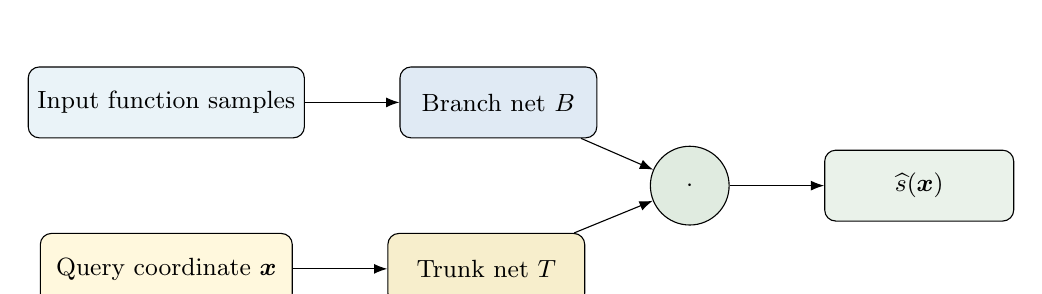
\begin{tikzpicture}[node distance=1.2cm,>=Latex,every node/.style={font=\small}]
\node[draw,rounded corners,fill=lightblue,minimum width=3.2cm,minimum height=0.9cm] (bf) {Input function samples};
\node[draw,rounded corners,fill=blue!15,right=of bf,minimum width=2.5cm,minimum height=0.9cm] (branch) {Branch net $B$};
\node[draw,rounded corners,fill=lightgold,below=1.2cm of bf,minimum width=3.2cm,minimum height=0.9cm] (xy) {Query coordinate $\vect{x}$};
\node[draw,rounded corners,fill=gold!20,right=of xy,minimum width=2.5cm,minimum height=0.9cm] (trunk) {Trunk net $T$};
\node[draw,circle,fill=green!15,right=2.0cm of $(branch)!0.5!(trunk)$,minimum size=1.0cm] (dot) {$\cdot$};
\node[draw,rounded corners,fill=green!10,right=of dot,minimum width=2.4cm,minimum height=0.9cm] (out) {$\widehat{s}(\vect{x})$};
\draw[->] (bf)--(branch); \draw[->] (xy)--(trunk);
\draw[->] (branch)--(dot); \draw[->] (trunk)--(dot); \draw[->] (dot)--(out);
\end{tikzpicture}
\end{center}

\subsection{What we implement in Week 4}
The class notebook uses Reynolds number in the branch and $(x,y)$ in the trunk:
\begin{equation}
B(\widetilde{\Rey}),\qquad T(x,y)\quad\longrightarrow\quad (u,v).
\end{equation}
This is a \textbf{parameterized DeepONet-style architecture}. It is useful for learning a parametric solution family, but it is not a full demonstration of learning an arbitrary input function. A genuine cavity operator-learning dataset could vary the lid profile $U_{lid}(x)$; the branch would receive sensor values $[U_{lid}(\xi_1),\ldots,U_{lid}(\xi_m)]$.

\begin{warningbox}
Do not claim operator generalization from a dataset that varies only one scalar parameter. The architecture may be DeepONet-like, but the scientific claim is parameter-to-field generalization.
\end{warningbox}

\section{Comparing Coordinate DNN and DeepONet}
The coordinate DNN mixes parameters and coordinates at its input. DeepONet keeps a separate representation of the case and the query location, then combines latent features. This separation can be beneficial when many functions and coordinates are available, but no architecture is guaranteed to win on a small dataset.

\begin{center}
\begin{tabular}{p{0.25\textwidth}p{0.31\textwidth}p{0.31\textwidth}}
\toprule
Property & Coordinate DNN & DeepONet-style model\\
\midrule
Inputs & $(\Rey,x,y)$ together & branch: $\Rey$; trunk: $(x,y)$\\
Output & $(u,v)$ & latent inner products for $(u,v)$\\
Natural strength & simple neural field & separated case/coordinate encoding\\
Key risk & local fit without topology & overclaiming operator learning\\
Required baseline & field interpolation & field interpolation and coordinate DNN\\
\bottomrule
\end{tabular}
\end{center}

\section{Metrics for Fields}
For a predicted velocity field,
\begin{equation}
E_{uv}=\frac{\sqrt{\sum_j[(\hat u_j-u_j)^2+(\hat v_j-v_j)^2]}}
{\sqrt{\sum_j[u_j^2+v_j^2]}}.
\end{equation}
Also report component MAE, maximum vector error, centerline error, wall-zone error, and inference time. Global metrics must be paired with physical checks.

\subsection{Physical validation}
\begin{align}
E_{div}&=\left[\frac{1}{N_{int}}\sum_{int}\left(\frac{\partial \hat u}{\partial x}+\frac{\partial \hat v}{\partial y}\right)^2\right]^{1/2},\\
E_{lid}&=\frac{1}{N_{lid}}\sum_{lid}|\hat u-1|,\\
E_{wall,n}&=\frac{1}{N_{wall}}\sum_{wall}|\hat{\vect{u}}\cdot\vect{n}|.
\end{align}
Inspect centerlines, streamlines, vortex displacement, and corner zones. A low global error can coexist with a wrong secondary vortex or severe boundary error.

\section{Interpolation, Extrapolation, and Uncertainty}
Interpolation asks for a Reynolds number inside the training range and bracketed by training cases. Extrapolation asks for a condition outside the observed range. DNNs do not automatically respect scaling laws outside training data. A responsible report must label every test as interpolation or extrapolation.

An ensemble of independently initialized models provides a simple uncertainty indicator. Ensemble spread is not a rigorous confidence interval, but large disagreement can flag difficult regions. Calibration must be tested against actual errors.

\section{Connection to Week 5: From Data Loss to Physics Loss}
Week 4 trains
\begin{equation}
\mathcal{L}=\mathcal{L}_{data}.
\end{equation}
Week 5 introduces
\begin{equation}
\mathcal{L}=\lambda_d\mathcal{L}_{data}+\lambda_{bc}\mathcal{L}_{bc}
+\lambda_{mom}\mathcal{L}_{momentum}+\lambda_{div}\mathcal{L}_{divergence}.
\end{equation}
The transition is conceptually important: a supervised model imitates labels; a PINN or physics-regularized model additionally penalizes violation of known equations or constraints. Competing loss components can train at different rates, so loss weighting is a genuine optimization issue, not a cosmetic choice.

\section{Recommended Week-4 Workflow}
\begin{enumerate}
\item Run and qualify the common $\Rey=100$ CFD case.
\item Generate one assigned production field.
\item Merge only accepted cases and freeze the dataset.
\item Extract scalar vortex observables.
\item Fit interpolation and polynomial baselines.
\item Fit a compact scalar DNN.
\item Build a field-interpolation baseline.
\item Compare coordinate DNN and parameterized DeepONet-style models.
\item Freeze models and evaluate blind cases.
\item Report numerical errors, physical checks, and failures.
\end{enumerate}

\section{Common Failure Modes}
\begin{longtable}{p{0.25\textwidth}p{0.34\textwidth}p{0.31\textwidth}}
\toprule
Symptom & Likely cause & Required response\\
\midrule
Very small test error & Grid-point leakage & Split by complete Reynolds-number case\\
DNN worse than interpolation & Insufficient data or overfitting & Report baseline honestly; simplify model\\
Good interior, poor walls & Loss dominated by interior points & Add wall metrics; consider zonal sampling\\
Wrong streamlines, modest $L_2$ & Metric hides topology & Plot streamlines and vortex location\\
Excellent training, poor blind test & Memorization & Case-level cross-validation and smaller model\\
Unstable DeepONet result & Sparse function/case coverage & Reduce claim; repeat seeds; expand data\\
\bottomrule
\end{longtable}

\section{Summary}
\begin{itemize}
\item Data quality is part of the ML method.
\item The split must be by flow case, not by grid point.
\item Interpolation is a serious baseline for a one-parameter cavity family.
\item Numerical error and physical validity are different questions.
\item A coordinate DNN learns a neural field; DeepONet separates case and coordinate representations.
\item A scalar-parameter branch gives a DeepONet-style parametric surrogate, not full function-to-function operator learning.
\item Week 5 adds physics constraints and PINNs to the same cavity problem.
\end{itemize}

\section*{References}
\begin{enumerate}
\item U. Ghia, K. N. Ghia, and C. T. Shin, ``High-Re solutions for incompressible flow using the Navier--Stokes equations and a multigrid method,'' \emph{Journal of Computational Physics}, 48, 387--411, 1982.
\item L. Lu, P. Jin, and G. E. Karniadakis, ``DeepONet: Learning nonlinear operators for identifying differential equations based on the universal approximation theorem of operators,'' \emph{Nature Machine Intelligence}, 3, 218--229, 2021.
\item M. Raissi, P. Perdikaris, and G. E. Karniadakis, ``Physics-informed neural networks: A deep learning framework for solving forward and inverse problems involving nonlinear partial differential equations,'' \emph{Journal of Computational Physics}, 378, 686--707, 2019.
\item S. Wang, X. Yu, and P. Perdikaris, ``When and why PINNs fail to train: A neural tangent kernel perspective,'' \emph{Journal of Computational Physics}, 449, 110768, 2022.
\end{enumerate}

\end{document}
